\documentclass[10pt,a4paper,twocolumn]{article}

\usepackage[utf8]{inputenc}
\usepackage[T1]{fontenc}
\usepackage[spanish,activeacute]{babel}
\usepackage{lmodern}
\usepackage{geometry}
\usepackage{graphicx}
\usepackage{xcolor}
\usepackage{amsmath, amssymb}
\usepackage{array}
\usepackage{booktabs}
\usepackage{enumitem}
\usepackage{float}
\usepackage{placeins}
\usepackage{caption}
\usepackage{dblfloatfix}
\usepackage{tikz}
\usetikzlibrary{positioning, arrows.meta, fit, calc, babel}
\usepackage[hidelinks]{hyperref}

\geometry{left=1.8cm, right=1.8cm, top=2.2cm, bottom=2.2cm}
\setlength{\columnsep}{0.75cm}

\DeclareMathOperator{\sen}{sen}
\DeclareMathOperator{\sgn}{sgn}

\setlist[itemize]{leftmargin=1.2em, noitemsep, topsep=2pt}
\setlist[enumerate]{leftmargin=1.6em, noitemsep, topsep=2pt}

\captionsetup{font=small, labelfont=bf}

\renewcommand{\topfraction}{0.9}
\renewcommand{\dbltopfraction}{0.9}
\renewcommand{\textfraction}{0.07}
\renewcommand{\floatpagefraction}{0.8}
\renewcommand{\dblfloatpagefraction}{0.5}
\setcounter{topnumber}{3}
\setcounter{dbltopnumber}{2}

% marca visual para los datos que faltan por completar
\newcommand{\pend}[1]{\textcolor{red}{\textbf{[#1]}}}

\begin{document}

% ---------------------------------------------------------------- PORTADA
\onecolumn
\begin{center}
\rule{\linewidth}{0.5mm}\\[0.4cm]
\par\vspace{0.25cm}
\Huge\textbf{Taller 6\\[0.15cm]}
\Large\textbf{Sistema Eléctrico -- Rotacional -- Traslación}
\par\vspace{0.5cm}
\rule{\linewidth}{0.5mm}\\[5.0cm]

\vspace{2cm}
\Large{
\begin{tabular}{rl}
\textbf{Fecha}        & 26-10-2026 \\[4pt]
\textbf{Integrantes}  & \begin{tabular}[t]{@{}l@{}} Vicente Andrade \\ Ignacio Godoy \end{tabular} \\[10pt]
\textbf{Grupo}        & 3 \\[4pt]
\textbf{Asignatura}   & Dinámica de Procesos Industriales \\[4pt]
\textbf{Profesor}     & Alejandro Suárez \\
\end{tabular}
}
\end{center}
\clearpage

% ---------------------------------------------------------------- CUERPO
\twocolumn

\section*{Descripción del sistema}

Se modela un ascensor duple de desplazamiento diagonal: dos cabinas que recorren rieles
paralelos de inclinación $\theta$, unidas por un cable que pasa por la rueda (tambor) de la
estación superior. Cada extremo del cable baja por un lado de la rueda hasta una cabina,
de modo que cuando la rueda gira una cabina sube y la otra baja: es un funicular
\emph{contrapesado}, como los ascensores de Valparaíso, en que el peso de una cabina
equilibra el de la otra. En la Fig.~2 del enunciado ambas cabinas aparecen en la mitad del
recorrido, que es justamente el punto en que se cruzan.

La rueda es accionada por el mismo sistema de potencia rotacional del Taller 3: motor de
corriente continua, eje del motor con torsión, juego de engranajes reductor y eje
secundario con torsión. Lo nuevo está en los dos extremos de la cadena:
\begin{itemize}
  \item \textbf{Entrada.} El motor ya no se excita con un voltaje continuo $V(t)$, sino a
        través de un rectificador trifásico alimentado por un voltaje \emph{monofásico}
        alterno $V_s(t)$. Para que una sola fase pueda excitar un rectificador trifásico
        se intercala un convertidor AC--AC (monofásico a trifásico). El voltaje en el
        motor, $U(t)$, pasa a ser una variable interna: es la que piden graficar las
        preguntas 3 y 4.
  \item \textbf{Carga.} La rueda ya no arrastra una cabina sino dos, unidas por el cable.
        Cada cabina es idéntica a la del Taller 2 sin roce seco: masa, peso proyectado,
        roce viscoso en todo el recorrido y amortiguadores en ambos extremos de su riel.
\end{itemize}
La variable a observar es la velocidad de las cabinas.

\subsection*{Criterios de modelamiento}

Los apuntes de clase sobre modelado físico dan los criterios con que se construye el
modelo. Se indica para cada uno dónde se aplica:
\begin{itemize}
  \item \textbf{Efectos pequeños, según con qué se comparen.} La caída en directo de un
        diodo ($\approx1$ V) frente a los $\approx420$ V del bus es un $0{,}25$\,\% y se
        desprecia (H2). La masa del cable se desprecia frente a la de las cabinas (H6).
  \item \textbf{Cada subsistema tiene sus propias aproximaciones.} El eléctrico (diodos
        ideales, convertidor ideal), el rotacional (las del Taller 3) y el traslacional
        (las del Taller 2) se aproximan por separado y se unen en sus puertas.
  \item \textbf{Distintas escalas de tiempo.} El sistema va desde la torsión del eje del
        motor (período de $3{,}7$ ms) hasta el viaje ($64$ s). Se cuantifica en la Fase 3.
  \item \textbf{Lo más simple es eliminar variables de estado; idealmente
        $\tau_{max}/\tau_{min}\le 10$--$100$.} Las dinámicas muy rápidas se aproximan por
        relaciones estáticas: así se obtiene el \emph{modelo promedio} de la Fase 3, con el
        rectificador promediado y los ejes rígidos, que se usa para diseñar la excitación.
        Las muy lentas se aproximan por constantes: temperaturas, y con ello $R_a$, y masas
        de pasajeros (H11).
  \item \textbf{Agrupación de variables de estado.} Los acumuladores que comparten el
        mismo flujo se juntan en uno: rueda y cabinas en una sola inercia $J_{eq}$, y los
        resortes de los topes que actúan a la vez en uno solo por extremo (punto 11). El
        rizado del rectificador se reemplaza por su promedio en un período.
  \item \textbf{Ecuaciones en derivadas parciales $\to$ bloques concentrados.} El cable y
        los ejes son elementos distribuidos; se representan por bloques donde se acumula y
        se propaga la energía: torsiones $K_1$ y $K_2$ con inercias concentradas, y cable
        rígido.
  \item \textbf{Convección} (dos medios distintos). Corresponde al enfriamiento del motor
        y de los diodos. Es una dinámica de minutos y no se modela (H11).
  \item \textbf{Bloque \emph{function} para el convertidor AC--AC y el rectificador.} Se
        implementan en Simulink con bloques \emph{MATLAB Function} (punto 14).
\end{itemize}

\subsection*{Hipótesis de modelamiento}

\begin{itemize}
  \item[\textbf{H1}] El convertidor AC--AC es ideal: no tiene pérdidas ni dinámica propia, y
        entrega un sistema trifásico equilibrado de secuencia positiva, de la misma
        frecuencia que $V_s$ y amplitud $a$ veces la de $V_s$. Lo construye con la
        transformada inversa de Clarke a partir de dos componentes: $v_\alpha = V_s(t)$ y
        $v_\beta = V_s(t-T/4)$, que es la misma tensión retrasada en $90^\circ$. Es válido
        mientras la amplitud de $V_s$ varíe lentamente frente a $T = 20$ ms.
  \item[\textbf{H2}] Los tres diodos son ideales, de cátodo común (rectificador de media onda
        de tres pulsos), y cada uno va en serie con la resistencia $R_s$ de su fase
        (devanado y resistencia dinámica del diodo). Se desprecian la caída en directo y las
        inductancias de conmutación. El neutro del convertidor es el polo negativo del bus.
  \item[\textbf{H3}] El condensador del bus $C$ es ideal: sin resistencia serie ni fuga.
  \item[\textbf{H4}] Motor de CC de excitación independiente y flujo constante, con $R_a$ y
        $L_a$ en serie con la fuerza contraelectromotriz (H1 y H2 del Taller 3).
  \item[\textbf{H5}] El sistema de potencia rotacional es idéntico al del Taller 3: engranajes
        ideales, cuya inercia está incluida en $J_2$, y roces viscosos concentrados en
        $\beta_1$ y $\beta_2$.
  \item[\textbf{H6}] El cable no tiene masa y es inextensible: es un transmisor rígido. Ambas
        cabinas quedan ligadas a la rueda, $v_A = r\,\omega_p$ y $v_B = -v_A$. Al no tener
        masa el cable, el desequilibrio de pesos no depende de la posición.
  \item[\textbf{H7}] Cada cable solo tracciona: $F_A \ge 0$ y $F_B \ge 0$. Es una
        restricción que se verifica sobre la salida.
  \item[\textbf{H8}] Las cabinas son las del Taller 2: masa constante durante el viaje (los
        pasajeros no se mueven), peso proyectado, roce viscoso $\gamma$ en todo el riel
        (\textbf{sin roce seco}) y amortiguadores unilaterales en ambos extremos. Se trabaja
        en condición seca, sin lluvia.
  \item[\textbf{H9}] Los dos rieles son iguales, paralelos y de igual largo $x_S$, con las
        estaciones alineadas. La posición de $B$ medida desde su estación inferior es
        $x_B = x_S - x_A$: cuando $A$ toca su tope superior, $B$ toca a la vez su tope
        inferior, y viceversa.
  \item[\textbf{H10}] Es positivo el sentido de giro que hace subir la cabina $A$. El sentido
        de marcha se elige con un contactor inversor de la armadura, que no se modela. Como
        las cabinas son iguales, todo viaje equivale a uno en que sube $A$, intercambiando
        las masas.
  \item[\textbf{H11}] Los efectos térmicos (calentamiento, convección) son mucho más lentos
        que un viaje: los parámetros eléctricos se toman constantes.
  \item[\textbf{H12}] El freno mecánico del tambor retiene las cabinas en las estaciones. Se
        libera en $t=0$, con todo el sistema en reposo, y vuelve a actuar al término del
        viaje; no se modela.
\end{itemize}

\begin{figure*}[p]
\centering
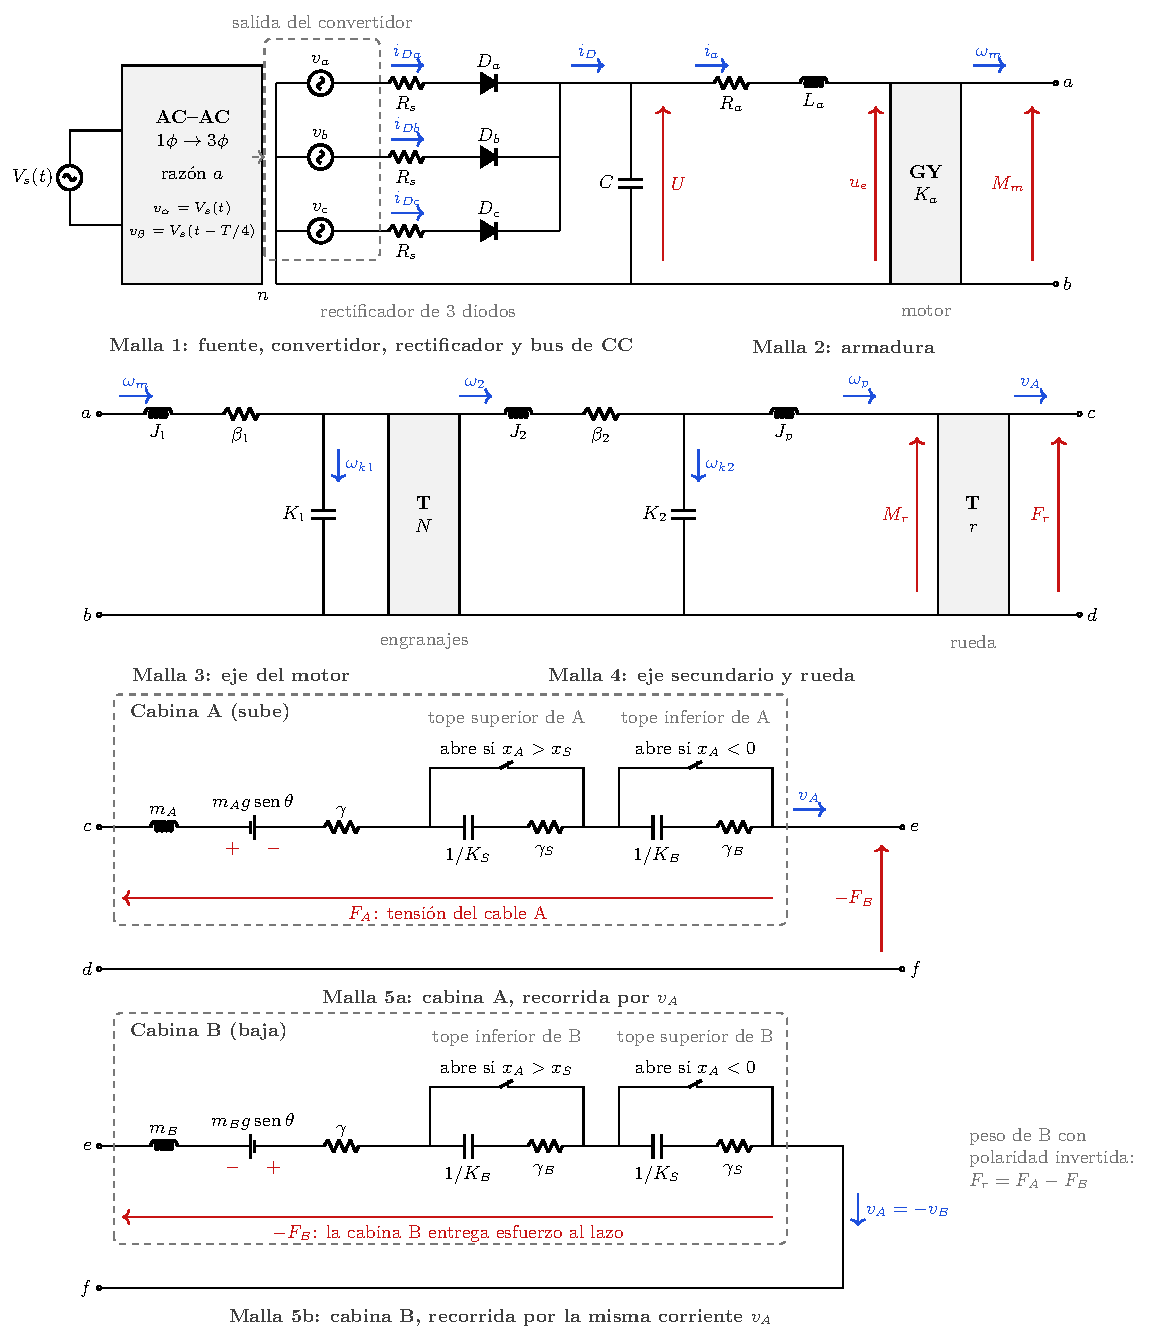
\includegraphics[width=\textwidth]{figuras/circuito_equivalente.pdf}
\caption{Diagrama simbólico eléctrico equivalente del sistema completo (pregunta 5),
con la analogía esfuerzo--voltaje. Es un solo circuito, dibujado en cuatro tramos unidos
por los terminales $a$--$b$, $c$--$d$ y $e$--$f$. Las flechas azules son flujos
(corrientes, velocidades) y las rojas, esfuerzos (voltajes, torques, fuerzas). El
convertidor AC--AC entrega tres fuentes alternas en estrella; cada una alimenta el bus a
través de $R_s$ y de su diodo, y el condensador $C$ fija el voltaje del motor $U$. Las dos
cabinas quedan en serie, recorridas por la misma corriente $v_A=-v_B$: la cabina $B$
aparece con su peso de polaridad invertida, de modo que $F_r = F_A - F_B$. Cada
amortiguador está puenteado por un interruptor cerrado que se abre durante el contacto
con su tope.}
\label{fig:eq}
\end{figure*}

% ================================================================ FASE 1
\section*{Fase 1. Estructurando el problema}

\subsection*{1.- Variable de entrada al sistema total}
\begin{itemize}
  \item $V_s(t) = \sqrt{2}\,V_{ef}(t)\,\sen(2\pi f t)$: voltaje monofásico $[\mathrm{V}]$,
        de frecuencia $f = 50$ Hz y valor eficaz $V_{ef}(t)$
\end{itemize}

\subsection*{2.- Variables a observar del sistema total}
\begin{itemize}
  \item $v_A(t)$, $v_B(t) =$ Velocidades de las cabinas $[\mathrm{m/s}]$, salida pedida
  \item $x_A(t)$, $x_B(t) =$ Posiciones de las cabinas $[\mathrm{m}]$, que gobiernan el
        contacto con los amortiguadores
  \item $U(t) =$ Voltaje en el motor $[\mathrm{V}]$, pedido en las preguntas 3 y 4
  \item $i_a(t) =$ Corriente de armadura $[\mathrm{A}]$
  \item $F_A(t)$, $F_B(t) =$ Tensiones de los cables $[\mathrm{N}]$, para verificar H7
\end{itemize}

\subsection*{3.- Componentes del sistema}
\begin{itemize}
  \item Fuente de voltaje monofásica.
  \item Convertidor AC--AC monofásico a trifásico, con razón $a$.
  \item Rectificador: tres resistencias de fase $R_s$ y tres diodos.
  \item Condensador del bus de CC, $C$.
  \item Circuito de armadura $R_a$, $L_a$ y motor de CC como girador.
  \item Eje del motor ($J_1$, $\beta_1$, $K_1$), engranajes ($N$), eje secundario ($J_2$,
        $\beta_2$, $K_2$) y rueda ($J_p$, $r$), iguales al Taller 3.
  \item Dos cabinas, cada una con masa, peso proyectado, roce viscoso y dos amortiguadores
        de extremo con sus conmutadores.
\end{itemize}

\subsection*{4.- Variables internas}

\noindent\textbf{Malla 1 (fuente, convertidor, rectificador y bus)}
\begin{itemize}
  \item $v_\alpha(t),\ v_\beta(t) =$ Componentes de entrada del convertidor $[\mathrm{V}]$
  \item $v_a(t),\ v_b(t),\ v_c(t) =$ Tensiones de fase del convertidor $[\mathrm{V}]$
  \item $i_{Da}(t),\ i_{Db}(t),\ i_{Dc}(t) =$ Corrientes de los diodos $[\mathrm{A}]$
  \item $i_D(t) =$ Corriente total del rectificador $[\mathrm{A}]$
  \item $U(t),\ i_C(t) =$ Voltaje y corriente del condensador del bus
\end{itemize}

\noindent\textbf{Malla 2 (armadura)}
\begin{itemize}
  \item $i_a(t),\ u_{Ra}(t),\ u_{La}(t),\ u_e(t)$, como en el Taller 3
\end{itemize}

\noindent\textbf{Mallas 3 y 4 (ejes y rueda).} Las mismas del Taller 3: $M_m$,
$\omega_m$, $M_{J1}$, $M_{\beta1}$, $M_{k1}$, $\omega_{k1}$, $M_1$, $\omega_1$, $M_2$,
$\omega_2$, $M_{J2}$, $M_{\beta2}$, $M_{k2}$, $\omega_{k2}$, $M_p$, $\omega_p$, $M_{Jp}$ y
$M_r$.

\noindent\textbf{Malla 5 (cabinas)}
\begin{itemize}
  \item $F_r(t) = F_A(t) - F_B(t) =$ Fuerza neta de los cables sobre la rueda $[\mathrm{N}]$
  \item $F_{mA},\ F_{mB} =$ Fuerzas de las masas de las cabinas $[\mathrm{N}]$
  \item $F_{gA},\ F_{gB} =$ Pesos proyectados sobre el riel $[\mathrm{N}]$
  \item $F_{\gamma A},\ F_{\gamma B} =$ Fuerzas del roce viscoso $[\mathrm{N}]$
  \item $F_{kSA},\ F_{kBA},\ F_{kSB},\ F_{kBB} =$ Fuerzas de los resortes de los topes
        superior (S) e inferior (B) de cada cabina $[\mathrm{N}]$
  \item $F_{amA},\ F_{amB} =$ Fuerza total de los amortiguadores de cada cabina $[\mathrm{N}]$
  \item $s_2(t),\ s_3(t) =$ Estados de los conmutadores $[-]$
\end{itemize}

\noindent\textbf{Momentos y carga}
\begin{itemize}
  \item $p_{J1},\ p_{J2},\ p_{Jp} =$ Momentos angulares $[\mathrm{Nms}]$
  \item $p_A,\ p_B =$ Momentos lineales de las cabinas $[\mathrm{kg\,m/s}]$
  \item $q_C =$ Carga del condensador del bus $[\mathrm{C}]$
\end{itemize}

\subsection*{5.- Constantes}
\begin{itemize}
  \item $f$, $T = 1/f =$ Frecuencia y período de la red $[\mathrm{Hz}]$, $[\mathrm{s}]$
  \item $a =$ Razón de amplitud del convertidor AC--AC $[-]$
  \item $R_s =$ Resistencia serie de cada fase del rectificador $[\Omega]$
  \item $C =$ Capacidad del condensador del bus $[\mathrm{F}]$
  \item $R_a$, $L_a$, $K_a$, $J_1$, $\beta_1$, $K_1$, $N$, $J_2$, $\beta_2$, $K_2$, $J_p$,
        $r$: las del Taller 3, con las mismas unidades
  \item $m_A$, $m_B =$ Masas de las cabinas con pasajeros $[\mathrm{kg}]$
  \item $g$, $\theta$, $\gamma$, $K_S$, $\gamma_S$, $K_B$, $\gamma_B$, $x_S$: las del
        Taller 2, iguales para ambas cabinas
\end{itemize}

\noindent Se mantienen las convenciones del Taller 3: $K_1$ y $K_2$ son flexibilidades
$[\mathrm{rad/Nm}]$ (condensador $C=K$), mientras que $K_S$ y $K_B$ son rigideces
$[\mathrm{N/m}]$ (condensador $C=1/K$); la razón de engranajes cumple $M_2=N M_1$ y
$\omega_1 = N\omega_2$.

\subsection*{6.- Equivalente eléctrico}

Se usa la analogía esfuerzo--voltaje del Taller 3, extendida a la nueva entrada y a la
nueva carga. El resultado es el diagrama simbólico de la Fig.~\ref{fig:eq}, que responde a
la pregunta 5.

La \textbf{malla 1} es eléctrica real y sigue el esquema de la pizarra: tres fuentes
alternas con un diodo cada una y un condensador a la salida. Las tres fuentes $v_a$, $v_b$,
$v_c$ son la salida del convertidor AC--AC, conectadas en estrella con neutro común $n$.
Cada fase alimenta el bus a través de su resistencia $R_s$ y de su diodo; los tres cátodos
se unen en el polo positivo. El condensador $C$ conecta el polo positivo con el neutro, y su
voltaje es el del motor, $U$.

Las \textbf{mallas 2 a 4} son las del Taller 3: la armadura, el girador $K_a$, los ejes con
sus inercias (inductores), roces (resistores) y torsiones (condensadores en derivación), y
los transformadores de los engranajes y de la rueda.

La \textbf{malla 5} es la carga nueva, y es donde mejor se ve el efecto del contrapeso.
Por la rueda, cuya razón es $r$, circula la velocidad $v_A$; como el cable es rígido, la
cabina $B$ lleva la velocidad $v_B=-v_A$. Escritas con la corriente común $v_A$, las fuerzas
de $B$ cambian de signo:
\begin{gather*}
  -F_{mB} = m_B\,\dot v_A, \qquad -F_{\gamma B} = \gamma\,v_A \\
  -F_{gB} = -m_B\,g\sen\theta
\end{gather*}
La inercia y el roce de $B$ siguen siendo un inductor y un resistor en serie con los de
$A$, pero su peso es una batería de \emph{polaridad invertida}. Ambas cabinas quedan
entonces en serie (tramos 5a y 5b de la figura, unidos por $e$--$f$), y las dos baterías
se restan: con cargas iguales se anulan. Sobre la cabina $A$ cae el esfuerzo $F_A$; sobre
la $B$, $-F_B$: la cabina que baja \emph{entrega} esfuerzo al lazo, que es justamente el
efecto del contrapeso. Los amortiguadores también quedan en serie: cuando $A$ toca su tope
superior, $B$ toca el inferior, y los dos condensadores $1/K_S$ y $1/K_B$ entran a la vez.

% ================================================================ FASE 2
\section*{Fase 2. Estableciendo las ecuaciones básicas}

\subsection*{7.- Leyes de los componentes}

\noindent\textbf{Convertidor AC--AC} (transformada inversa de Clarke)
\begin{align*}
  v_\alpha &= V_s(t), \qquad v_\beta = V_s(t - T/4) \\
  v_a &= a\,v_\alpha \\
  v_b &= a\big(-\tfrac12 v_\alpha + \tfrac{\sqrt3}{2} v_\beta\big) \\
  v_c &= a\big(-\tfrac12 v_\alpha - \tfrac{\sqrt3}{2} v_\beta\big)
\end{align*}
Con $V_s = \sqrt2 V_{ef}\sen\omega t$ resulta $v_k = \sqrt2\,a V_{ef}
\sen(\omega t - \varphi_k)$, con $\varphi_k = 0,\ 120^\circ,\ 240^\circ$.

\noindent\textbf{Diodos con resistencia de fase}, $k\in\{a,b,c\}$
\[
  i_{Dk} = \frac{1}{R_s}\max\big(0,\ v_k - U\big)
\]

\noindent\textbf{Condensador del bus}
\[
  i_C = C\,\frac{dU}{dt}
\]

\noindent\textbf{Armadura, girador y sistema rotacional:} las leyes del punto 7 del
Taller 3, con $U$ en lugar de $V$:
\begin{align*}
  u_{Ra} &= R_a i_a, \quad u_{La} = L_a \tfrac{di_a}{dt} \\
  u_e &= K_a\omega_m, \quad M_m = K_a i_a \\
  M_{J1} &= J_1\dot\omega_m,\ \ M_{J2} = J_2\dot\omega_2,\ \ M_{Jp} = J_p\dot\omega_p \\
  M_{\beta1} &= \beta_1\omega_m, \quad M_{\beta2} = \beta_2\omega_2 \\
  \omega_{k1} &= K_1 \dot M_{k1}, \quad \omega_{k2} = K_2 \dot M_{k2} \\
  M_2 &= N M_1, \quad \omega_1 = N\omega_2 \\
  M_r &= r F_r, \quad v_A = r\,\omega_p
\end{align*}

\noindent\textbf{Cabinas}, $j\in\{A,B\}$
\begin{align*}
  F_{mj} &= m_j\,\dot v_j, \quad F_{gj} = m_j g\sen\theta, \quad F_{\gamma j} = \gamma\,v_j \\
  \dot F_{kSj} &= K_S\,s_{Sj}\,v_j, \quad \dot F_{kBj} = K_B\,s_{Bj}\,v_j
\end{align*}
y los roces de los amortiguadores $\gamma_S v_j$ y $\gamma_B v_j$ durante el contacto.

\noindent\textbf{Conmutadores.} Por H9, los cuatro contactos dependen solo de $x_A$:
\begin{align*}
  s_2 &= s_{SA} = s_{BB} = \begin{cases} 1 & x_A > x_S \\ 0 & \text{si no} \end{cases} \\
  s_3 &= s_{BA} = s_{SB} = \begin{cases} 1 & x_A < 0 \\ 0 & \text{si no} \end{cases}
\end{align*}

\subsection*{8.- Leyes de conexión}

\noindent\textbf{Malla 1} (nodo del polo positivo)
\[
  i_D = i_{Da} + i_{Db} + i_{Dc}, \qquad i_C = i_D - i_a
\]

\noindent\textbf{Malla 2}
\[
  U = u_{Ra} + u_{La} + u_e
\]

\noindent\textbf{Mallas 3 y 4:} las del Taller 3,
\begin{align*}
  M_m &= M_{J1} + M_{\beta1} + M_{k1}, \quad M_1 = M_{k1} \\
  \omega_{k1} &= \omega_m - \omega_1, \quad \omega_{k2} = \omega_2 - \omega_p \\
  M_2 &= M_{J2} + M_{\beta2} + M_{k2} \\
  M_{k2} &= M_{Jp} + M_r
\end{align*}

\noindent\textbf{Malla 5}
\begin{align*}
  v_A &= r\,\omega_p, \qquad v_B = -v_A \\
  F_A &= F_{mA} + F_{gA} + F_{\gamma A} + F_{amA} \\
  F_B &= F_{mB} + F_{gB} + F_{\gamma B} + F_{amB} \\
  F_r &= F_A - F_B
\end{align*}
con $F_{amj} = s_{Sj}(F_{kSj} + \gamma_S v_j) + s_{Bj}(F_{kBj} + \gamma_B v_j)$. La última
ecuación expresa que los dos cables tiran de la rueda por lados opuestos: el de $A$
resiste el giro positivo y el de $B$ lo favorece.

\subsection*{9.- Leyes de conservación}

\noindent a) Conservación de la carga en el nodo del bus:
\[
  \frac{dq_C}{dt} = i_D - i_a
\]

\noindent b) Conservación del momento angular: las tres ecuaciones del Taller 3, con
$\dot p_{Jp} = M_{k2} - r(F_A - F_B)$.

\noindent c) Conservación del momento lineal en cada cabina:
\begin{align*}
  \dot p_A &= F_A - F_{gA} - F_{\gamma A} - F_{amA} \\
  \dot p_B &= F_B - F_{gB} - F_{\gamma B} - F_{amB}
\end{align*}

\subsection*{10.- Relaciones físicas}

\noindent Momentos y carga:
\[
  p_{Jk} = J_k\,\omega_k, \quad p_j = m_j v_j, \quad q_C = C\,U
\]

\noindent Posiciones:
\[
  \frac{dx_A}{dt} = v_A, \qquad x_B = x_S - x_A
\]

\noindent Deformación de los resortes durante el contacto, como en el Taller 3:
\begin{align*}
  F_{kSA} &= K_S(x_A - x_S) \ge 0, & F_{kBB} &= K_B\,x_B \le 0 \\
  F_{kBA} &= K_B\,x_A \le 0,       & F_{kSB} &= K_S(x_B - x_S) \ge 0
\end{align*}

\noindent Restricciones de validez:
\[
  F_A \ge 0, \qquad F_B \ge 0, \qquad i_{Dk} \ge 0
\]
Las dos primeras corresponden a H7. La tercera no es una hipótesis sino la física del
diodo, y tiene una consecuencia central: \textbf{el rectificador no puede devolver energía
a la red}. La corriente del bus solo entra, de modo que el motor puede traccionar pero no
frenar regenerando. Esto define la Fase 4.

% ================================================================ FASE 3
\section*{Fase 3. Modelamiento del sistema}

\subsection*{11.- Variables de estado}

Los elementos que acumulan energía son trece: $C$, $L_a$, $J_1$, $K_1$, $J_2$, $K_2$,
$J_p$, $m_A$, $m_B$ y los cuatro resortes de los topes. No todos son independientes, y aquí
se aplica la \emph{agrupación de variables de estado}:
\begin{itemize}
  \item \textbf{Inercias.} $J_p$, $m_A$ y $m_B$ están ligadas por el cable rígido: en el
        equivalente son tres inductores con la misma corriente, a través del
        transformador $r$. Se agrupan reflejando ambas cabinas al eje de la rueda:
        \begin{equation}
          J_{eq} = J_p + (m_A + m_B)\,r^2
          \label{eq:Jeq}
        \end{equation}
        Las cabinas \emph{suman} su inercia aunque sus pesos se resten.
  \item \textbf{Topes.} Por H9, el tope superior de $A$ y el inferior de $B$ actúan
        siempre juntos, con la misma corriente $v_A$. Son dos condensadores en serie, que
        equivalen a una rigidez $K_e = K_S + K_B$ y a un roce $\gamma_e = \gamma_S +
        \gamma_B$. Lo mismo ocurre con el tope inferior de $A$ y el superior de $B$. Se
        definen así dos fuerzas de resorte agrupadas:
        \[
          F_{kS} = F_{kSA} - F_{kBB} \ge 0, \qquad F_{kI} = F_{kBA} - F_{kSB} \le 0
        \]
\end{itemize}
Quedan nueve acumuladores independientes. Igual que en los Talleres 2 y 3, se agrega la
posición $x_A$, que gobierna los conmutadores:
\begin{enumerate}
  \item $U$: voltaje del condensador del bus, es decir, el voltaje en el motor.
  \item $i_a$: corriente de armadura.
  \item $\omega_m$: velocidad del rotor ($J_1$).
  \item $M_{k1}$: torque en la torsión $K_1$.
  \item $\omega_2$: velocidad del eje secundario ($J_2$).
  \item $M_{k2}$: torque en la torsión $K_2$.
  \item $\omega_p$: velocidad de la rueda con ambas cabinas ($J_{eq}$).
  \item $F_{kS}$: resortes del contacto superior de $A$ (inferior de $B$).
  \item $F_{kI}$: resortes del contacto inferior de $A$ (superior de $B$).
  \item $x_A$: posición de la cabina $A$.
\end{enumerate}
\[
  x(t) = \big[\, U,\ i_a,\ \omega_m,\ M_{k1},\ \omega_2,\ M_{k2},\ \omega_p,\ F_{kS},\
  F_{kI},\ x_A \,\big]^{T}
\]
con condiciones iniciales nulas: bus descargado, ejes sin carga y cabina $A$ en reposo en
la estación inferior, con $B$ en la superior (H12).

\noindent\textbf{Observaciones.}
\begin{itemize}
  \item El retardo $T/4$ del convertidor no es una variable de estado: forma parte de la
        fuente. Las tensiones $v_a$, $v_b$, $v_c$ se tratan como entradas conocidas,
        funciones de $V_s(t)$.
  \item Como en el Taller 3, la realización es no mínima: durante el contacto $F_{kS}$ y
        $F_{kI}$ quedan determinadas por $x_A$. Se conservan como estados para respetar el
        criterio de un estado por acumulador.
  \item La agrupación de los topes no es una aproximación: es exacta porque ambos
        contactos ocurren en el mismo instante.
\end{itemize}

\subsection*{12.- Derivadas en función de las variables de estado}

Reemplazando las leyes de los componentes en las de conexión:
\begin{align}
  \frac{dU}{dt}       &= \frac{1}{C}\big[\, i_D - i_a \,\big] \tag{12.1}\label{eq:x1}\\
  \frac{di_a}{dt}     &= \frac{1}{L_a}\big[\, U - R_a i_a - K_a\omega_m \,\big] \tag{12.2}\\
  \frac{d\omega_m}{dt}&= \frac{1}{J_1}\big[\, K_a i_a - \beta_1\omega_m - M_{k1} \,\big] \tag{12.3}\\
  \frac{dM_{k1}}{dt}  &= \frac{1}{K_1}\big[\, \omega_m - N\omega_2 \,\big] \tag{12.4}\\
  \frac{d\omega_2}{dt}&= \frac{1}{J_2}\big[\, N M_{k1} - \beta_2\omega_2 - M_{k2} \,\big] \tag{12.5}\\
  \frac{dM_{k2}}{dt}  &= \frac{1}{K_2}\big[\, \omega_2 - \omega_p \,\big] \tag{12.6}\\
  \frac{d\omega_p}{dt}&= \frac{1}{J_{eq}}\big[\, M_{k2} - r F_c \,\big] \tag{12.7}\label{eq:x7}\\
  \frac{dF_{kS}}{dt}  &= K_e\, s_2(x_A)\, r\,\omega_p \tag{12.8}\\
  \frac{dF_{kI}}{dt}  &= K_e\, s_3(x_A)\, r\,\omega_p \tag{12.9}\\
  \frac{dx_A}{dt}     &= r\,\omega_p \tag{12.10}\label{eq:x10}
\end{align}
donde la corriente del rectificador y la fuerza resistente de la carga son
\begin{align*}
  i_D &= \frac{1}{R_s}\sum_{k=a,b,c}\max\big(0,\ v_k(t) - U\big) \\
  F_c &= F_g + 2\gamma\, r\omega_p + s_2\big[F_{kS} + \gamma_e r\omega_p\big]
       + s_3\big[F_{kI} + \gamma_e r\omega_p\big] \\
  F_g &= (m_A - m_B)\, g\sen\theta
\end{align*}
La fuerza $F_c$ contiene toda la diferencia con el Taller 3. El peso aparece solo a través
del \emph{desequilibrio} $m_A - m_B$, mientras que el roce de las dos cabinas se suma. Con
cargas equilibradas, el motor solo debe vencer roces.

\noindent\textbf{Estructura.} El sistema es lineal a trozos. Hay dos fuentes de no
linealidad: la conmutación de los diodos, que depende de $U$ y de $t$, y la de los topes,
que depende de $x_A$. Para cada combinación de diodos en conducción y de contactos, las diez
ecuaciones son lineales afines.

\subsection*{13.- Salidas en función de las variables de estado}
\begin{align}
  y_1 &= v_A = r\,\omega_p, \qquad y_2 = v_B = -r\,\omega_p \tag{13.1}\\
  y_3 &= x_A, \qquad\qquad\ \ y_4 = x_B = x_S - x_A \tag{13.2}\\
  y_5 &= U, \qquad\qquad\ \ \ y_6 = i_a \tag{13.3}\\
  y_7 &= F_A = m_A(\dot v_A + g\sen\theta) + \gamma v_A + F_{amA} \tag{13.4}\\
  y_8 &= F_B = m_B(g\sen\theta - \dot v_A) - \gamma v_A + F_{amB} \tag{13.5}
\end{align}
con $\dot v_A = r\,\dot\omega_p$ tomado de \eqref{eq:x7}. Durante el contacto, las fuerzas
agrupadas $F_{kS}$ y $F_{kI}$ se reparten entre los dos topes en proporción a su rigidez.

\subsection*{Escalas de tiempo y modelo promedio}

Linealizando el núcleo del modelo, con el rectificador reemplazado por su conductancia
media, y agregando los tiempos propios de la fuente, se obtienen las escalas de la
Tabla~\ref{tab:escalas}.

\begin{table}[H]
\centering
\caption{Escalas de tiempo del sistema completo (cargas equilibradas).}
\label{tab:escalas}
\small
\begin{tabular}{@{}lr@{}}
\toprule
Fenómeno & Escala \\
\midrule
Carga de $C$ por un diodo, $R_sC$                     & $2$ ms \\
Torsión del eje del motor ($\zeta = 0{,}001$)        & $3{,}7$ ms \\
Rizado del rectificador, $T/3$ (150 Hz)               & $6{,}7$ ms \\
Armadura, $L_a/R_a$                                   & $16$ ms \\
Período de la red, $T$                                & $20$ ms \\
Modo bus--armadura ($\zeta = 0{,}64$), período        & $57$ ms \\
Modo electromecánico, $\tau$                          & $0{,}14$ s \\
Torsión del eje secundario ($\zeta = 0{,}13$)        & $0{,}17$ s \\
Rodado libre sin corriente, $\tau_m$                  & $3{,}1$ s \\
Rampas de aceleración y frenado                      & $8$--$20$ s \\
Viaje completo                                        & $64$ s \\
\bottomrule
\end{tabular}
\end{table}

La razón $\tau_{max}/\tau_{min} \approx 64/0{,}002 \approx 3\times10^{4}$ está muy por
encima del rango de 10 a 100 recomendado en clase. Para la pregunta que interesa, la
velocidad de las cabinas a lo largo de un viaje, todo lo que ocurre bajo los 20 ms puede
tratarse como estático:
\begin{itemize}
  \item \textbf{Ejes rígidos.} Se eliminan $M_{k1}$ y $M_{k2}$ y se refiere todo al eje del
        motor:
        \begin{align*}
          J_{tot} &= J_1 + \frac{J_2 + J_{eq}}{N^2} = 0{,}852\ \mathrm{Nms^2} \\
          c_m     &= \beta_1 + \frac{\beta_2 + 2\gamma r^2}{N^2} = 0{,}271\ \mathrm{Nms/rad}
        \end{align*}
        Referidos al riel, equivalen a una masa de $m_{eq} = J_{tot}(N/r)^2 = 5452$ kg y a un
        roce de $c = c_m (N/r)^2 = 1736$ Ns/m. Del total, $2240$ kg corresponden al rotor del
        motor.
  \item \textbf{Rectificador promedio.} Si el condensador mantiene $U$ casi constante
        durante un período, cada diodo conduce mientras $V_m\cos\vartheta > U$, es decir en
        $|\vartheta|<\vartheta_c$, con $V_m = \sqrt2\,aV_{ef}$. Promediando la corriente de
        las tres fases:
        \begin{align}
          \bar i_D &= \frac{3}{\pi R_s}\big(V_m\sen\vartheta_c - U\vartheta_c\big),
          \quad U = V_m\cos\vartheta_c \notag\\
          &\Rightarrow\ \tan\vartheta_c - \vartheta_c = \frac{\pi R_s\, \bar i_D}{3\,U}
          \label{eq:rect}
        \end{align}
        Es una relación estática entre $V_m$, $U$ y la corriente media. Con carga nula
        $U = V_m$: el bus se carga al valor peak.
\end{itemize}
Lo que queda es un modelo de primer orden en $\omega_m$, cuya única constante de tiempo
mecánica es la de rodado libre, $\tau_m = J_{tot}/c_m = 3{,}1$ s, y la electromecánica,
$J_{tot}R_a/K_a^2 = 63$ ms. Su razón es 50, dentro del rango de clase. Este \emph{modelo
promedio} se usa para diseñar la excitación por dinámica inversa (punto 15), y el modelo
completo de diez estados se usa para verificar el diseño.

\noindent\textbf{Ley de régimen permanente.} En régimen todas las derivadas del modelo se
anulan, y para una velocidad constante $v$ se obtiene
\begin{align}
  U &= A\,v + B\,(m_A - m_B) \label{eq:ley}\\
  A &= \frac{K_a N}{r} + \frac{R_a N}{K_a r}\,c_m = 212{,}17\ \mathrm{Vs/m} \notag\\
  B &= \frac{R_a\, r\, g\sen\theta}{K_a N} = 0{,}0118\ \mathrm{V/kg} \notag
\end{align}
y la corriente $i_a = \big(c_m N v/r + r(m_A-m_B)g\sen\theta/N\big)/K_a$. Comparada con la
ley del Taller 3, el término independiente ya no es el peso de la cabina sino el
desequilibrio. Además, $i_a\ge0$ exige
\begin{equation}
  m_B - m_A \le \frac{c_m N^2 v}{r^2 g\sen\theta} = \frac{c\,v}{g\sen\theta}
  \label{eq:lim}
\end{equation}
que vale $708$ kg a $2$ m/s. Si la cabina que baja supera a la que sube en más de esa masa,
la gravedad le gana al roce y el motor tendría que frenar. El rectificador de diodos no
puede hacerlo.

% ================================================================ FASE 4
\section*{Fase 4. Validación}

\subsection*{14.- Simulación}

\subsubsection*{Asignación de valores a los elementos (pregunta 2)}

Los valores del sistema rotacional se heredan del Taller 3 y los de las cabinas del Taller
2, sin cambios. Se dimensionan los elementos nuevos, la fuente, el convertidor y el
rectificador, y se definen las dos condiciones de carga (Tabla~\ref{tab:param}).

\begin{table*}[t]
\centering
\caption{Valores asignados a los elementos del sistema.}
\label{tab:param}
\small
\begin{tabular}{@{}l l l p{0.50\textwidth}@{}}
\toprule
\textbf{Constante} & \textbf{Valor} & \textbf{Unidad} & \textbf{Justificación} \\
\midrule
\multicolumn{4}{@{}l}{\textit{Elementos nuevos (Taller 6)}}\\
$f$        & $50$               & Hz       & Frecuencia de la red chilena. \\
$V_n$      & $220$              & V rms    & Tensión monofásica nominal; $V_s$ se ajusta bajo este valor. \\
$a$        & $1{,}5$            & --       & Con $V_s = 220$ V el peak de fase es $467$ V, y por \eqref{eq:rect} el bus entrega $431$ V a la corriente nominal del motor del Taller 3 ($44$ A): cubre el peor caso, $431$ V a $31$ A en el Ensayo 2a. \\
$R_s$      & $0{,}2$            & $\Omega$ & Resistencia de devanado y diodo, $\approx 1{,}5$\,\% de la impedancia base de fase; limita los pulsos de carga del condensador a $\sim100$ A. \\
$C$        & $10$               & mF       & Rizado acotado por $\Delta U \le \bar i_D/(3fC) = 11$ V pico a pico a $17$ A (resulta $8$ V, un $2$\,\%, porque el condensador se descarga solo mientras ningún diodo conduce). El filtro $C$--$L_a$ queda en $112$ rad/s, muy bajo los $942$ rad/s del rizado. \\
$m_{vacía}$ & $1200$            & kg       & Cabina sin pasajeros. \\
$m_{llena}$ & $1800$            & kg       & Capacidad de 8 pasajeros de $75$ kg (masa por persona de la norma de ascensores). \\
$m_C$      & $1500$             & kg       & Carga media (4 pasajeros), igual a la del Taller 2; se usa en ambas cabinas para el caso equilibrado. \\
$J_{eq}$   & $800$              & Nms$^2$  & Calculada con \eqref{eq:Jeq}; vale lo mismo en todos los ensayos, pues $m_A + m_B = 3000$ kg. \\
\midrule
\multicolumn{4}{@{}l}{\textit{Sistema rotacional, heredado del Taller 3}}\\
$R_a$, $L_a$, $K_a$ & $0{,}5$; $8\times10^{-3}$; $2{,}6$ & $\Omega$; H; Vs/rad & Motor de $440$ V, $44$ A, $160$ rad/s. \\
$J_1$, $\beta_1$, $K_1$ & $0{,}35$; $0{,}015$; $2\times10^{-4}$ & Nms$^2$; Nms/rad; rad/Nm & Rotor y eje rápido. \\
$N$        & $40$               & --       & Reducción $40{:}1$. \\
$J_2$, $\beta_2$, $K_2$ & $3$; $10$; $2\times10^{-6}$ & Nms$^2$; Nms/rad; rad/Nm & Engranaje secundario y eje lento. \\
$J_p$, $r$ & $50$; $0{,}5$      & Nms$^2$; m & Tambor de $1$ m de diámetro. \\
\midrule
\multicolumn{4}{@{}l}{\textit{Cabinas y recorrido, heredados del Taller 2 (sin roce seco)}}\\
$\theta$, $g$ & $\pi/6$; $9{,}81$ & rad; m/s$^2$ & Inclinación de $30^\circ$. \\
$\gamma$   & $800$              & Ns/m     & Roce viscoso de cada cabina, en todo su riel. \\
$K_S = K_B$ & $1{,}5\times10^{5}$ & N/m    & Rigidez de los amortiguadores. \\
$\gamma_S = \gamma_B$ & $29\,200$ & Ns/m   & Roce de los amortiguadores. \\
$x_S$      & $100$              & m        & Largo de cada riel. \\
\bottomrule
\end{tabular}
\end{table*}

Dos verificaciones de coherencia. La primera: con cargas equilibradas, la ley
\eqref{eq:ley} pide $424{,}3$ V a $2$ m/s, y \eqref{eq:rect} traduce ese valor en
$V_s = 208{,}6$ V rms, bajo los $220$ V nominales. La segunda: en el peor caso, la cabina
llena subiendo, se piden $216{,}5$ V rms y $30{,}8$ A, también dentro de lo nominal. El
motor del Taller 3, dimensionado para una cabina sola, queda holgado: el contrapeso le
quita casi todo el trabajo contra la gravedad.

\subsubsection*{Implementación en Simulink}

El modelo lo genera el script \texttt{construir\_modelo\_t6.m} directamente desde las
ecuaciones de estado \eqref{eq:x1}--\eqref{eq:x10}, como en el Taller 3: una fila
\emph{From $\rightarrow$ Gain $\rightarrow$ Sum $\rightarrow$ Gain $\rightarrow$
Integrator $\rightarrow$ Goto} por cada variable de estado. La Fig.~\ref{fig:slx}
muestra su estructura.

\begin{figure}[!t]
\centering
\begin{tikzpicture}[font=\scriptsize, >=Stealth,
  b/.style={draw, fill=gray!10, align=center, minimum height=0.8cm, inner sep=2pt},
  f/.style={draw, fill=yellow!15, align=center, minimum height=0.8cm, inner sep=2pt},
  e/.style={draw, fill=blue!6, align=left, inner sep=3pt, anchor=north west}]
\node[b, text width=1.5cm] (vef) at (0.85,0)    {From Workspace\\$V_{ef}(t)$};
\node[b, text width=1.5cm] (sin) at (0.85,-1.1) {Sine Wave\\$\sqrt2\,\sen\omega t$};
\node[b, minimum width=0.5cm] (prod) at (2.45,-0.55) {$\times$};
\node[b, text width=1.25cm] (del) at (3.95,-0.55) {Transport\\Delay $T/4$};
\node[f, text width=1.45cm] (conv) at (6.6,-0.55) {MATLAB Fcn\\convertidor\\AC--AC};
\node[f, text width=1.45cm] (rect) at (6.6,-2.3) {MATLAB Fcn\\rectificador};
\draw[->] (vef.east) -| (prod.north);
\draw[->] (sin.east) -| (prod.south);
\draw[->] (prod.east) -- node[pos=0.3, below]{$V_s$} (del.west);
\draw[->] (del.east) -- node[above]{$v_\beta$} ([yshift=-0.15cm]conv.west);
\draw[->] (2.95,-0.55) -- (2.95,0.3) -- node[above]{$v_\alpha$} (5.6,0.3) |- ([yshift=0.2cm]conv.west);
\draw[->] (conv.south) -- node[right]{$v_{abc}$} (rect.north);
\node[e, text width=4.3cm] (est) at (0,-3.15)
  {\textbf{Filas de estado} (12.1)--(12.10)\\[1pt]
   $\Sigma \to 1/C \to \int \to U$\\
   $\Sigma \to 1/L_a \to \int \to i_a$\\
   $\Sigma \to 1/J_1 \to \int \to \omega_m$\\
   \quad$\vdots$\\
   $\Sigma \to 1/J_{eq} \to \int \to \omega_p$\\
   Switch $\to K_e \to \int \to F_{kS},\ F_{kI}$\\
   $r\omega_p \to \int \to x_A$};
\node[e, text width=2.45cm] (car) at (5.3,-3.15)
  {\textbf{Carga} $F_c$\\[1pt]
   $F_g + 2\gamma v$\\
   $+$ Switch $x_A>x_S$\\
   $+$ Switch $x_A<0$\\[3pt]
   \textbf{To Workspace}\\
   $U, i_a, i_D, v, x_A$};
\draw[->] ([yshift=0.15cm]rect.west) -| node[pos=0.25, above]{$i_D$} (3.0,-3.15);
\draw[->] (4.2,-3.15) |- node[pos=0.75, below]{$U$} ([yshift=-0.2cm]rect.west);
\draw[<->] (est.east |- 0,-4.6) -- node[above]{$v$, $x_A$} node[below]{$F_c$} (car.west |- 0,-4.6);
\end{tikzpicture}
\caption{Estructura del modelo Simulink. El convertidor y el rectificador son bloques
\emph{MATLAB Function} cuyo código escribe \texttt{construir\_modelo\_t6.m}. Las
señales circulan entre filas con etiquetas
\texttt{Goto}/\texttt{From}. El diagrama completo generado está en la
Fig.~\ref{fig:slxfull}.}
\label{fig:slx}
\end{figure}

\begin{figure*}[p]
\centering
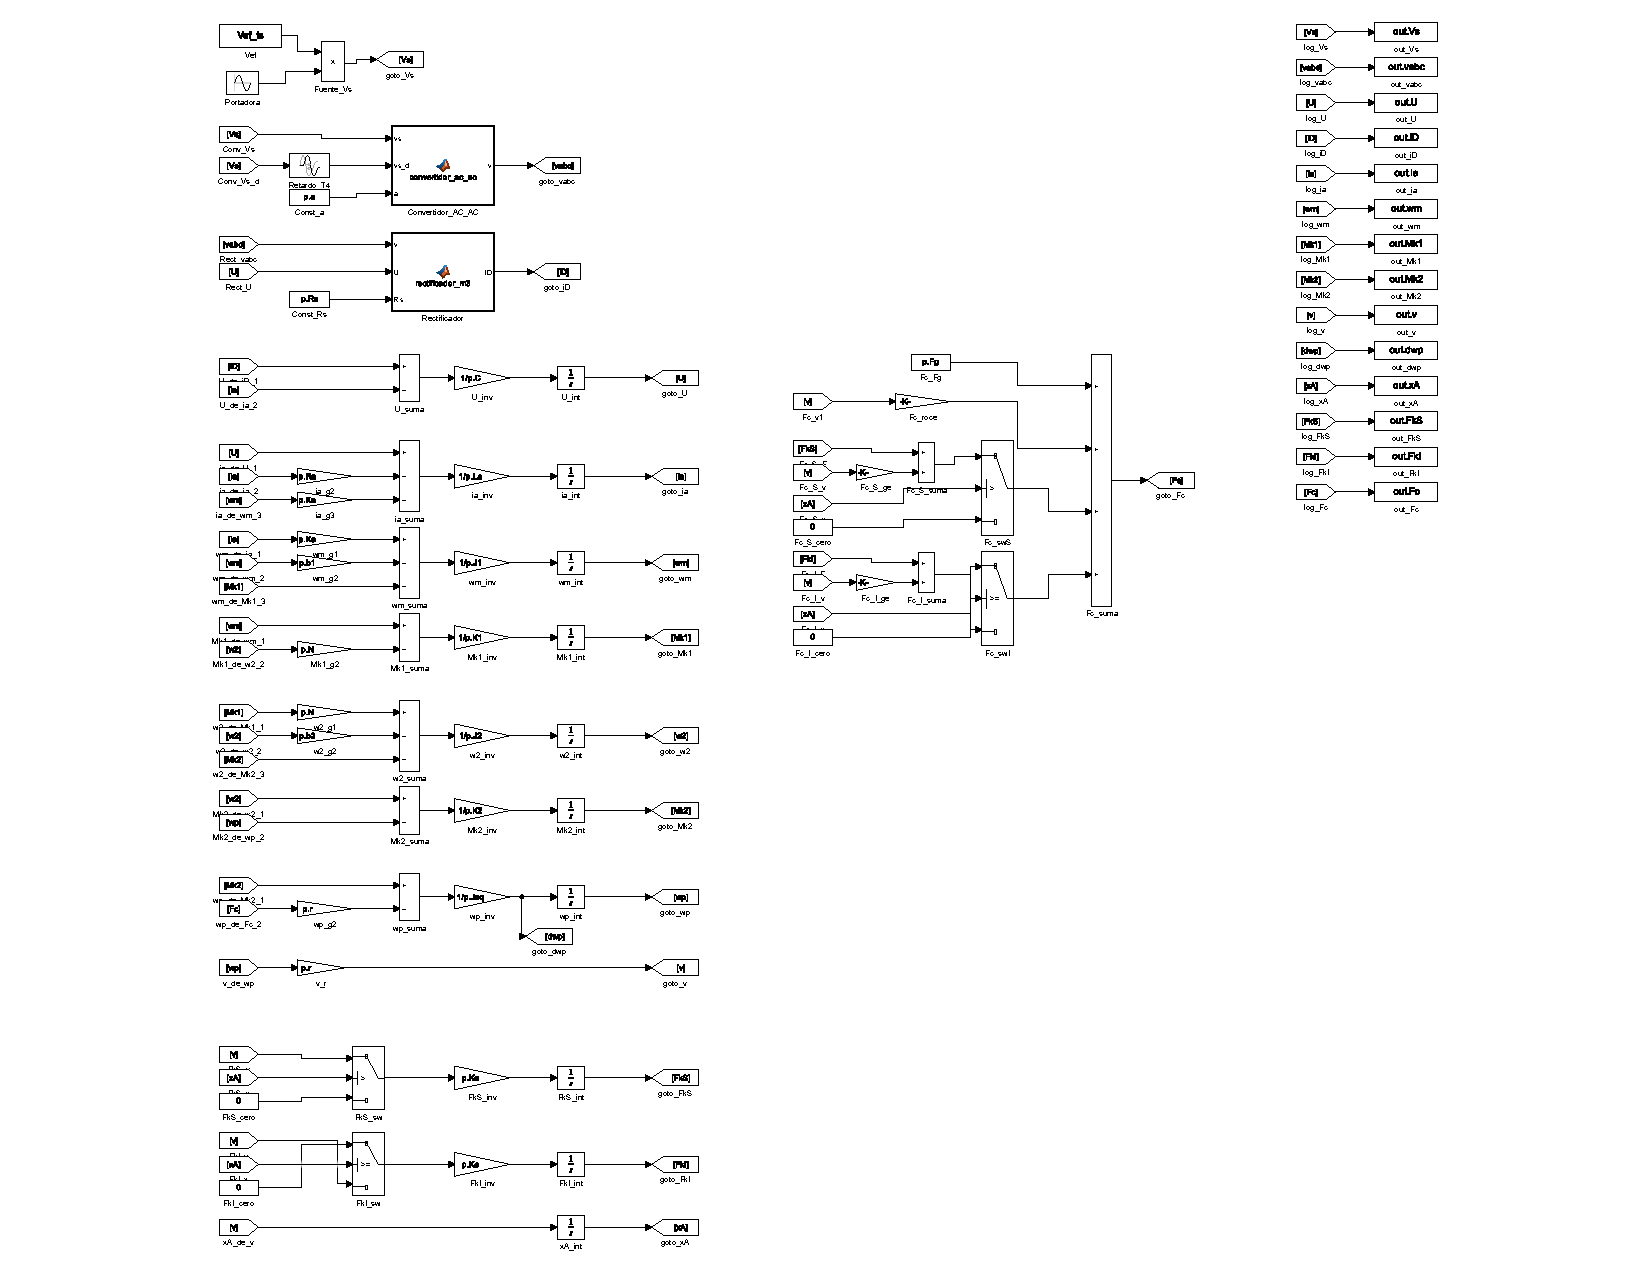
\includegraphics[trim=100 10 100 9, clip, width=0.92\textwidth]{figuras/diagrama_simulink.pdf}
\caption{Diagrama Simulink \texttt{ascensor\_duple\_t6.slx}, generado por
\texttt{construir\_modelo\_t6.m}. Arriba, la fuente $V_s(t)$, el \texttt{Transport Delay}
de $T/4$ y los bloques \emph{MATLAB Function} del convertidor AC--AC y del rectificador. A la
izquierda, las diez filas de las ecuaciones de estado (12.1)--(12.10), en el mismo orden del
punto 12. Al centro, la fuerza de la carga $F_c$ con los \texttt{Switch} de los topes. A la
derecha, el registro de señales con \texttt{To Workspace}.}
\label{fig:slxfull}
\end{figure*}

Los elementos nuevos respecto del Taller 3 son tres:
\begin{itemize}
  \item \textbf{Fuente.} $V_s(t)$ se forma con un bloque \texttt{Sine Wave} de amplitud
        $\sqrt2$, multiplicado por el valor eficaz $V_{ef}(t)$ que se lee con
        \texttt{From Workspace}. Así cada ensayo cambia solo la envolvente, sin tocar el
        diagrama.
  \item \textbf{Convertidor AC--AC.} Un \texttt{Transport Delay} de $T/4$ entrega
        $v_\beta$, y un bloque \emph{MATLAB Function} aplica la transformada inversa de
        Clarke para obtener $v_a$, $v_b$, $v_c$. Es el ``bloque \emph{function}'' sugerido
        en clase.
  \item \textbf{Rectificador.} Un segundo bloque \emph{MATLAB Function} recibe las tres
        fases y el voltaje del bus $U$, y devuelve $i_D$: suma las corrientes de los diodos
        que conducen. Su salida entra a la fila de $U$. Los diodos no necesitan bloques de
        potencia: su ley de componente es una función estática.
\end{itemize}
Las conmutaciones de los topes usan bloques \texttt{Switch} gobernados por $x_A$, como en
el Taller 3. Todos los parámetros se leen de la estructura \texttt{p}
(función \texttt{parametros\_t6} de \texttt{tests.m}). El script \texttt{tests.m}, que es
el único archivo necesario junto al \texttt{.slx}, carga en cada ensayo las masas y la
envolvente con \texttt{Simulink.SimulationInput}, sin modificar el modelo.

\noindent\textbf{Consideraciones numéricas.}
\begin{itemize}
  \item La separación de escalas de la Tabla~\ref{tab:escalas} hace al sistema rígido. Se
        usa \texttt{ode23t}, implícito y sin amortiguamiento numérico del modo de torsión,
        con paso máximo de $0{,}1$ ms, para resolver los pulsos de corriente de los diodos,
        que duran $\approx 1{,}8$ ms.
  \item Como verificación, \texttt{tests.m} integra también la ecuación de estado
        directamente, con su función \texttt{ecuacion\_estado\_t6} y RK4 de paso fijo de $0{,}1$ ms,
        y compara ambas soluciones. Los valores que se reportan en los ensayos (voltajes,
        corrientes y velocidades de crucero, posición de llegada y compresión de los topes)
        coinciden en las dos: el diagrama implementa las ecuaciones
        \eqref{eq:x1}--\eqref{eq:x10}.
\end{itemize}

\subsection*{15.- Ensayos}

Las figuras de esta sección son las que exporta \texttt{tests.m} a partir del modelo
Simulink.

\subsubsection*{Diseño de la excitación}

Igual que en el Taller 3, el voltaje no se elige: se diseña como \emph{perfil} por dinámica
inversa. Se propone la velocidad deseada $v^*(t)$ y se despeja hacia atrás, sobre el modelo
promedio:
\begin{align*}
  M_m^* &= J_{tot}\tfrac{N}{r}\dot v^* + c_m\tfrac{N}{r} v^* + \tfrac{r F_g}{N}, \qquad
  i_a^* = M_m^*/K_a \\
  U^* &= R_a i_a^* + L_a \dot i_a^* + K_a\tfrac{N}{r} v^*
\end{align*}
y con \eqref{eq:rect}, usando $\bar i_D = i_a^* + C\dot U^*$, se obtiene la amplitud $V_m^*$
y con ella $V_{ef}^* = V_m^*/(\sqrt2\,a)$. El perfil es la curva S de jerk continuo del
Taller 3: crucero a $v_c = 2$ m/s y rampa de aceleración de $T_a = 8$ s.

\textbf{La rampa de frenado debe ser más lenta que en el Taller 3}, por la restricción
$i_{Dk}\ge0$. Sin corriente, la cabina solo desacelera por roce, con $\tau_m = 3{,}1$ s, y
una rampa S que termina en reposo siempre exige al final una desaceleración mayor. La
Tabla~\ref{tab:frenado} muestra el compromiso para cargas equilibradas: la corriente
negativa que se necesitaría y la velocidad con que la cabina llega finalmente al tope.

\begin{table}[H]
\centering
\caption{Duración de la rampa de frenado, con cargas equilibradas.}
\label{tab:frenado}
\small
\begin{tabular}{@{}lccccc@{}}
\toprule
$T_d$ [s]                     & 8     & 12    & 16    & 20    & 24 \\
\midrule
$\min i_a^*$ [A]              & $-6{,}3$ & $-3{,}1$ & $-1{,}7$ & $-1{,}1$ & $-0{,}7$ \\
llegada [m/s]                 & $0{,}69$ & $0{,}42$ & $0{,}27$ & $0{,}17$ & $0{,}11$ \\
\bottomrule
\end{tabular}
\end{table}

Se adopta $T_d = 20$ s: la cabina se acopla al tope a $0{,}17$ m/s y el freno mecánico
completa la detención (H12). El viaje completo dura $64$ s, con $36$ s de crucero.

\subsubsection*{Ensayo 1: cargas equilibradas (pregunta 3)}

Ambas cabinas llevan $1500$ kg. La Fig.~\ref{fig:e1} muestra el voltaje en el motor que
produce el viaje a velocidad constante.

\begin{figure*}[!tp]
\centering
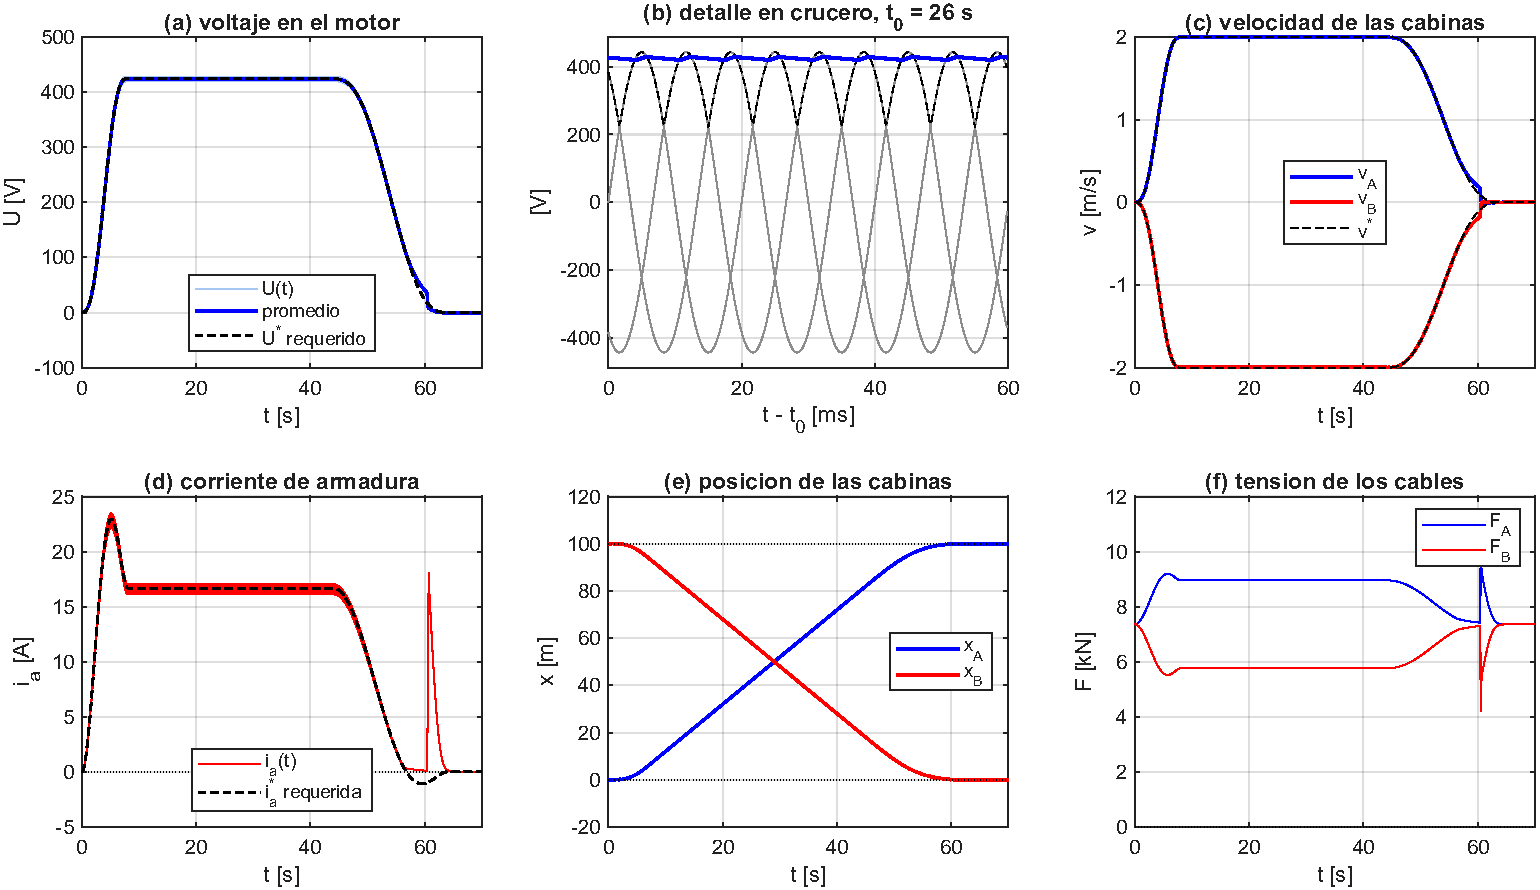
\includegraphics[width=\textwidth]{figuras/fig_ensayo1.pdf}
\caption{Ensayo 1, cargas equilibradas ($m_A = m_B = 1500$ kg). (a) Voltaje en el motor:
señal rectificada, su promedio en un período de rizado y el voltaje $U^*$ requerido por el
modelo promedio. (b) Detalle de tres períodos de red en crucero: tensiones de fase del
convertidor (gris), salida que tendría el rectificador sin condensador (segmentada) y
voltaje del bus $U$ (azul). (c)--(f) Velocidades, corriente, posiciones y tensiones de los
cables; en línea segmentada, los valores de diseño.}
\label{fig:e1}
\end{figure*}

En crucero el voltaje en el motor es \textbf{constante en promedio, $U = 424{,}0$ V}, y la
velocidad se mantiene en $v_A = -v_B = 1{,}9984$ m/s, $0{,}08$\,\% bajo la consigna.
Comentarios:
\begin{itemize}
  \item \textbf{El voltaje es constante porque los pesos se anulan.} Con $m_A = m_B$ la
        fuerza neta de gravedad sobre la rueda es nula: es la batería invertida de la
        Fig.~\ref{fig:eq}. El motor solo vence los roces, que a velocidad constante son
        constantes. Como el cable no tiene masa, el equilibrio se mantiene en todo el
        recorrido.
  \item \textbf{El voltaje lo fija la velocidad; la carga fija la corriente.} De los
        $424$ V, $416$ V son fuerza contraelectromotriz, $K_a N v/r$, y solo $8{,}3$ V son
        caída en $R_a$. Comparado con el Taller 3, de una cabina sin contrapeso, el voltaje
        baja apenas de $438$ a $424$ V, mientras que la corriente cae de $44$ a $16{,}7$ A y
        la potencia de $19{,}4$ a $7{,}1$ kW. Ese ahorro es la razón de ser del ascensor
        duple.
  \item \textbf{El voltaje real no es continuo puro.} El bus se carga en los peaks de las
        fases (panel b): cada diodo conduce $\approx 33^\circ$ por ciclo, con pulsos de
        $91$ A. El rizado es de $8{,}2$ V pico a pico ($419{,}9$ a $428{,}1$ V) a $150$ Hz.
        Sin condensador, el motor vería la envolvente de tres pulsos, que oscila entre
        $0{,}5\,V_m$ y $V_m$.
  \item \textbf{El rizado no llega a la velocidad.} Es la separación de escalas: el rizado
        de $6{,}7$ ms pasa por $L_a$, que lo reduce a $0{,}9$ A pico a pico en $i_a$, y por la
        inercia de $5452$ kg, cuya constante de tiempo es de segundos. En la velocidad
        queda una oscilación del orden de $10^{-7}$ m/s. Por eso el modelo promedio, que
        ignora el rizado, predice bien la velocidad.
  \item \textbf{Partida suave.} La corriente sigue al diseño con un peak de $23{,}5$ A
        durante la aceleración, frente a los $547$ A del escalón del Taller 3. El error de
        seguimiento en la rampa es de $4$ mm/s.
  \item \textbf{Frenado sin regeneración.} A partir de $t = 56{,}8$ s el diseño pide
        corriente negativa. Los diodos la bloquean, $i_a$ queda en cero (panel d), la cabina
        desacelera solo por roce y llega al tope a $0{,}17$ m/s, con $12$ mm de compresión.
\end{itemize}

\subsubsection*{Ensayo 2: cargas no equilibradas (pregunta 4)}

Se usa el desequilibrio de diseño: una cabina llena ($1800$ kg) y otra vacía ($1200$ kg),
$|\Delta m| = 600$ kg. Por H10 hay dos casos, según cuál cabina sube. La Fig.~\ref{fig:e2a}
los muestra con el mismo perfil del Ensayo 1, y la Fig.~\ref{fig:reg}
resume la ley \eqref{eq:ley} para todo desequilibrio.

\begin{figure*}[!tp]
\centering
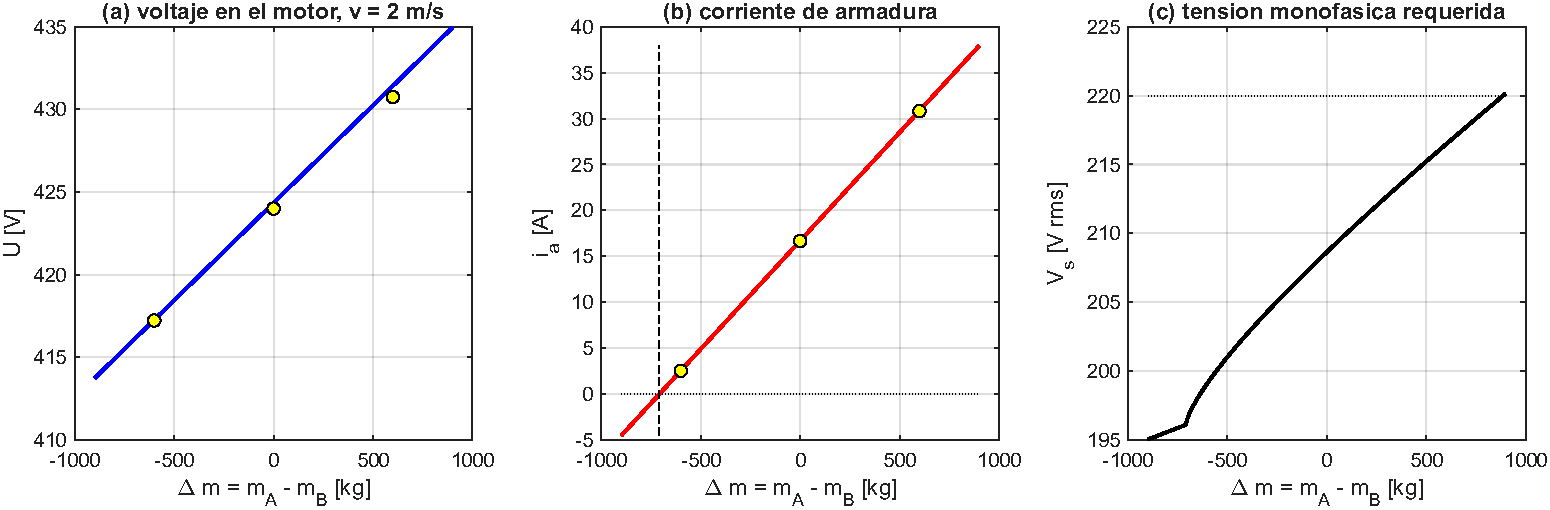
\includegraphics[width=\textwidth]{figuras/fig_regimen.pdf}
\caption{Ley de régimen permanente \eqref{eq:ley} a $v = 2$ m/s en función del
desequilibrio $\Delta m = m_A - m_B$, positivo cuando sube la cabina más pesada. Los
círculos son los valores medios simulados en crucero en los ensayos 1, 2a y 2b. La zona
gris de (b) exige corriente negativa, imposible con el rectificador de diodos.}
\label{fig:reg}
\end{figure*}

\begin{figure*}[p]
\centering
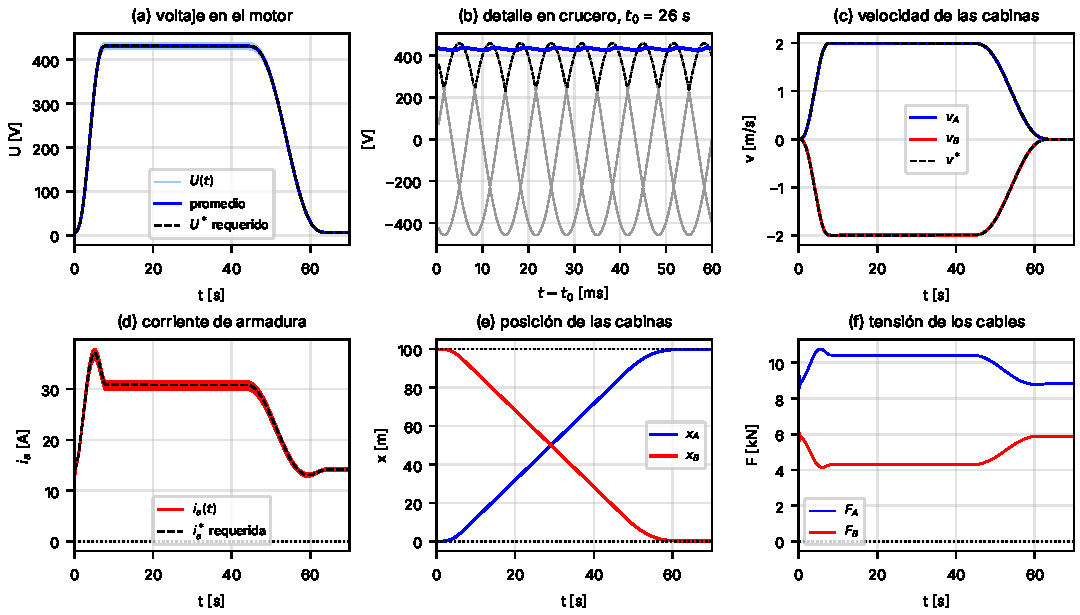
\includegraphics[width=\textwidth]{figuras/fig_ensayo2a.pdf}\\[4pt]
\small\textbf{(Ensayo 2a)} Cabina llena sube: $m_A = 1800$ kg, $m_B = 1200$ kg.\\[10pt]
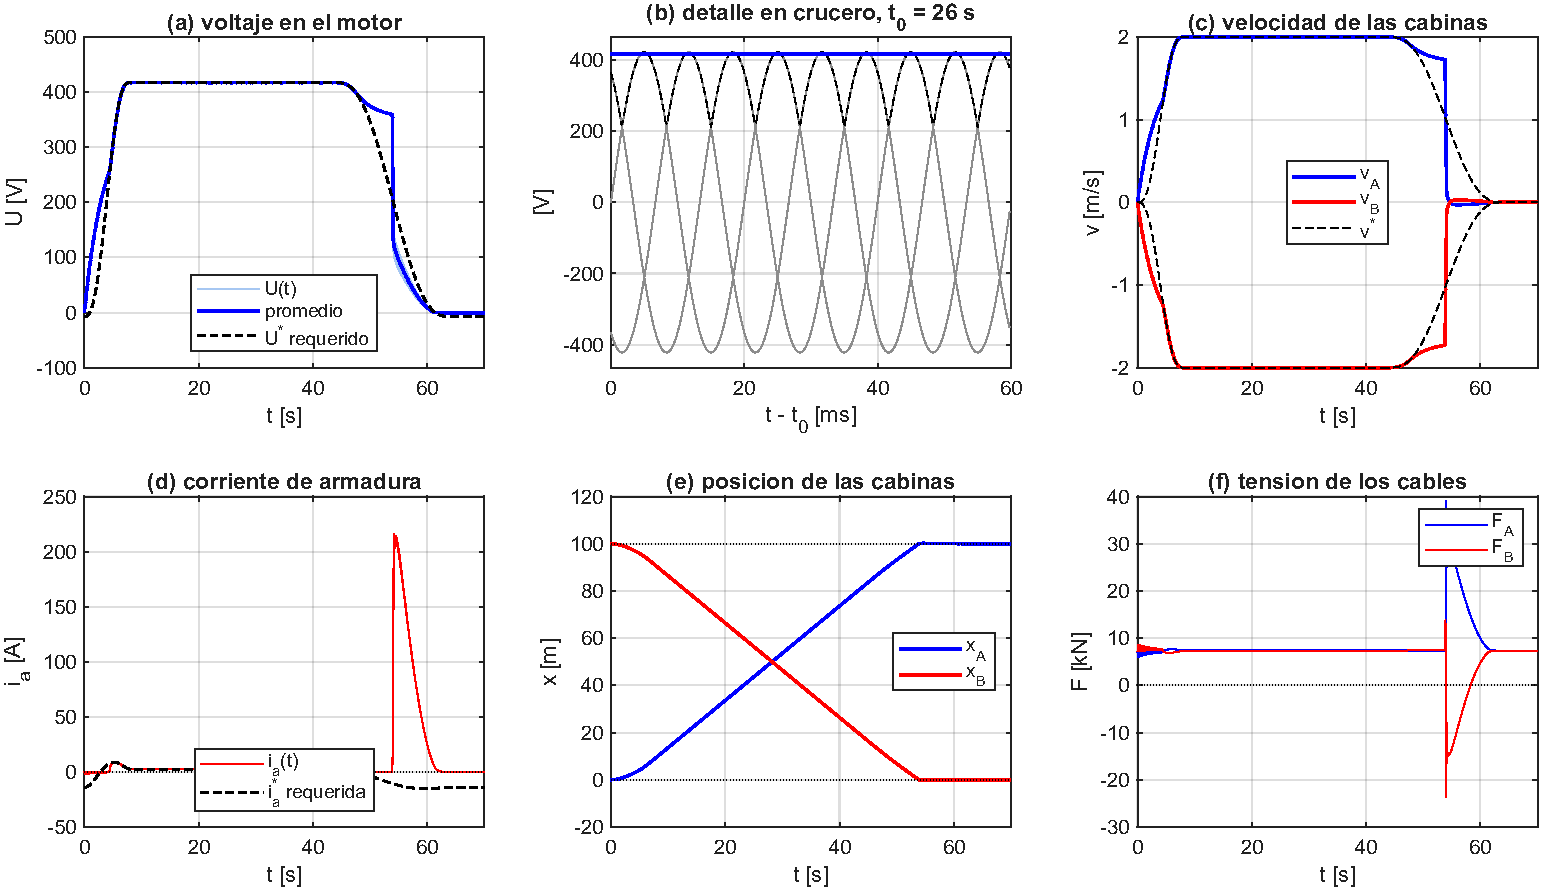
\includegraphics[width=\textwidth]{figuras/fig_ensayo2b.pdf}\\[4pt]
\small\textbf{(Ensayo 2b)} Cabina llena baja: $m_A = 1200$ kg, $m_B = 1800$ kg.
\caption{Ensayo 2, cargas no equilibradas, con los mismos paneles de la
Fig.~\ref{fig:e1}. En 2b el diseño pide corriente negativa al partir y al frenar, y el
rectificador no puede entregarla: la cabina se adelanta en la partida y no logra frenar,
y llega al tope a $1{,}72$ m/s.}
\label{fig:e2a}
\end{figure*}

\begin{center}
\small
\begin{tabular}{@{}lrrr@{}}
\toprule
Crucero a 2 m/s & \textbf{Equil.} & \textbf{2a} & \textbf{2b} \\
\midrule
$U$ medio [V]          & $424{,}0$ & $430{,}8$ & $417{,}2$ \\
Rizado de $U$ [V p-p]  & $8{,}2$   & $14{,}2$  & $1{,}4$ \\
$i_a$ medio [A]        & $16{,}7$  & $30{,}8$  & $2{,}5$ \\
$V_s$ requerido [V rms] & $208{,}6$ & $216{,}5$ & $199{,}1$ \\
$v_A$ medio [m/s]      & $1{,}9984$ & $1{,}9969$ & $1{,}9998$ \\
Potencia [kW]          & $7{,}1$   & $13{,}3$  & $1{,}1$ \\
\bottomrule
\end{tabular}
\end{center}

\noindent Comentarios:
\begin{itemize}
  \item \textbf{La velocidad constante se logra en ambos sentidos, con voltajes
        distintos.} $U = 430{,}8$ V cuando sube la cabina llena y $417{,}2$ V cuando baja:
        $\pm 7$ V respecto del caso equilibrado, la pendiente $B\,\Delta m$ de
        \eqref{eq:ley}. De nuevo la diferencia está en la corriente: $30{,}8$ A frente a
        $2{,}5$ A. El rizado crece con la corriente, porque el condensador se descarga más
        entre pulsos.
  \item \textbf{2a, cabina llena sube.} Es el caso exigente para el motor, pero el más
        favorable para el accionamiento: la corriente requerida es positiva en todo el
        viaje, entre $13$ y $37$ A, y el rectificador la entrega. La gravedad ayuda a frenar,
        así que la rampa de frenado se cumple sin rodado libre. Al final el motor retiene la
        cabina con $14{,}2$ A. Se detiene a $17$ cm de la estación: el error de $0{,}16$\,\%
        en la velocidad de crucero, debido a que el modelo promedio desprecia el rizado, se
        acumula a lo largo del viaje. Corregirlo exige medir la posición, es decir, cerrar el lazo.
  \item \textbf{2b, cabina llena baja.} En crucero el roce de las dos cabinas,
        $c\,v = 3472$ N, supera al desequilibrio, $\Delta m\, g\sen\theta = 2943$ N, y el
        motor aún tracciona con $2{,}5$ A: la velocidad se mantiene en $2{,}000$ m/s con el
        menor voltaje de los tres casos. A baja velocidad, en cambio, el roce desaparece y
        manda la gravedad. Al partir, el diseño pide corriente negativa durante $2{,}8$ s para
        retener la cabina; los diodos no lo permiten y el sistema se adelanta hasta
        $0{,}55$ m/s sobre el perfil y $1{,}6$ m en posición. Al frenar, el motor tampoco
        puede retener: la velocidad no baja de $v_\infty = \Delta m\, g\sen\theta/c =
        1{,}70$ m/s, en que la gravedad iguala al roce. La cabina llega al tope a
        $1{,}72$ m/s y lo comprime $157$ mm. Al calarse el motor contra el tope, el
        condensador se descarga en la armadura con un peak de $216$ A, y en el impacto el
        cable de $B$ se destensa ($F_B<0$): el modelo sale de su dominio de validez.
  \item \textbf{Límite del accionamiento.} El rectificador de diodos opera en un solo
        cuadrante, $U>0$ e $i_a>0$. Con la cabina pesada subiendo funciona siempre. Con la
        pesada bajando funciona solo en crucero, y solo si el desequilibrio es menor que el
        de \eqref{eq:lim}, $708$ kg a $2$ m/s: la capacidad de 8 pasajeros se eligió bajo
        ese valor. La partida, el frenado y la detención exigen en ese caso un elemento que
        absorba energía: el freno mecánico modulado, un \emph{chopper} con resistencia de
        frenado en el bus o un convertidor regenerativo, como un puente de tiristores en
        antiparalelo.
\end{itemize}

\subsubsection*{Diagrama simbólico eléctrico equivalente (pregunta 5)}

Es el de la Fig.~\ref{fig:eq}, desarrollado en el punto 6. Sus dos rasgos propios de este
taller son la malla 1, en que el rectificador aparece como tres fuentes con diodo sobre un
condensador común, y la malla 5, en que las cabinas quedan en serie con sus pesos opuestos.
Las agrupaciones del punto 11 se leen directamente en el circuito: inductores en serie con
la misma corriente ($J_{eq}$) y condensadores de los topes que entran a la vez ($K_e$).

\subsubsection*{Verificación de hipótesis y restricciones del modelo}

\begin{itemize}
  \item \textbf{H7, cables tensos.} En el recorrido útil, $F_A$ va de $6{,}0$ a $10{,}8$ kN
        y $F_B$ de $4{,}1$ a $8{,}6$ kN en los tres ensayos, siempre positivas. Solo se
        violan en el impacto del Ensayo 2b, fuera de la operación normal.
  \item \textbf{H1, envolvente lenta.} Las rampas de $V_{ef}$ duran de $8$ a $20$ s, frente
        a los $20$ ms del período: el convertidor ideal es aplicable.
  \item \textbf{Límites del equipo.} $V_s \le 216{,}5$ V rms, bajo los $220$ V nominales.
        $i_a\le 37{,}9$ A, bajo los $44$ A nominales del motor. Picos de diodo $\le 150$ A
        en operación normal.
  \item \textbf{Modelo promedio.} Predice el voltaje de crucero con error menor que $1$ V
        y la velocidad con error menor que $0{,}2$\,\%. Ignorar el rizado y la torsión para
        diseñar es legítimo, como anticipaba la separación de escalas.
  \item \textbf{Restricción $i_{Dk}\ge0$.} Es la que domina el comportamiento: obliga a
        alargar el frenado en el Ensayo 1 y hace inviable el Ensayo 2b fuera del crucero.
\end{itemize}

\end{document}
